% TRM error recovery 2x2 contingency matrix
% TransNAR Varied+/Varied+, n=1000
\begin{figure}[!t]
\centering
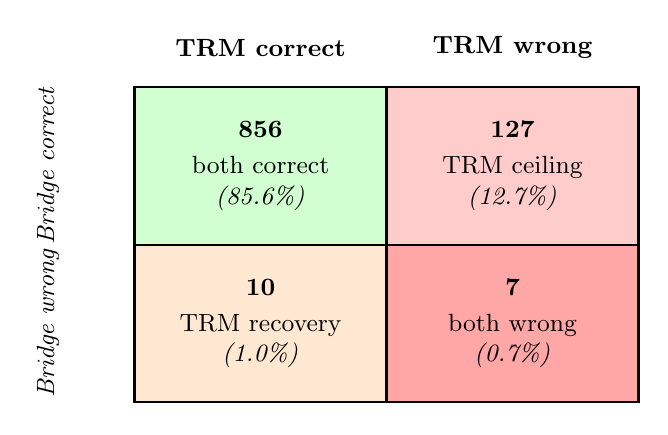
\begin{tikzpicture}[
    cell/.style={
        rectangle,
        draw=black,
        minimum width=3.2cm,
        minimum height=2.0cm,
        align=center,
        font=\small
    },
    header/.style={
        font=\small\bfseries,
        align=center
    },
    axislabel/.style={
        font=\small\itshape,
        align=center
    }
]

% Column headers
\node[header] at (1.6, 0.5)  {TRM correct};
\node[header] at (4.8, 0.5)  {TRM wrong};

% Row headers (rotated)
\node[axislabel, rotate=90] at (-1.1, -1.0) {Bridge correct};
\node[axislabel, rotate=90] at (-1.1, -3.0) {Bridge wrong};

% Top-left: B+T+ (856) -- both correct, lightest fill
\node[cell, fill=green!18] at (1.6, -1.0) {
    \textbf{856}\\[2pt]
    both correct\\
    \textit{(85.6\%)}
};

% Top-right: B+T- (127) -- bridge ok, TRM fails, medium fill
\node[cell, fill=red!20] at (4.8, -1.0) {
    \textbf{127}\\[2pt]
    TRM ceiling\\
    \textit{(12.7\%)}
};

% Bottom-left: B-T+ (10) -- bridge fails, TRM recovers, light fill
\node[cell, fill=orange!18] at (1.6, -3.0) {
    \textbf{10}\\[2pt]
    TRM recovery\\
    \textit{(1.0\%)}
};

% Bottom-right: B-T- (7) -- both fail, darkest fill
\node[cell, fill=red!35] at (4.8, -3.0) {
    \textbf{7}\\[2pt]
    both wrong\\
    \textit{(0.7\%)}
};

% Outer border
\draw[thick] (0, 0) rectangle (6.4, -4.0);
% Inner dividers
\draw[thick] (3.2, 0) -- (3.2, -4.0);
\draw[thick] (0, -2.0) -- (6.4, -2.0);

\end{tikzpicture}
\caption{Outcome breakdown for the TransNAR bridge trained on Varied+ data and evaluated on the Varied+ test set ($n=1000$). Rows indicate whether the bridge produced a correct grid; columns indicate whether TRM produced a correct solution. The dominant failure mode is B$^+$T$^-$: the bridge is correct but TRM fails, reflecting the solver's own accuracy ceiling. B$^-$T$^+$ cases (TRM recovers despite a bridge error) are rare and are analysed in the text.}
\label{fig:trm_recovery_matrix}
\end{figure}
